%%
%% This is file `tikzposter-template.tex',
%% generated with the docstrip utility.
%%
%% The original source files were:
%%
%% tikzposter.dtx  (with options: `tikzposter-template.tex')
%%
%% This is a generated file.
%%
%% Copyright (C) 2014 by Pascal Richter, Elena Botoeva, Richard Barnard, and Dirk Surmann
%%
%% This file may be distributed and/or modified under the
%% conditions of the LaTeX Project Public License, either
%% version 2.0 of this license or (at your option) any later
%% version. The latest version of this license is in:
%%
%% http://www.latex-project.org/lppl.txt
%%
%% and version 2.0 or later is part of all distributions of
%% LaTeX version 2013/12/01 or later.
%%


\documentclass{tikzposter} %Options for format can be included here

\usepackage{todonotes}

\usepackage[tikz]{bclogo}
\usepackage{lipsum}
\usepackage{amsmath}

\usepackage{booktabs}
\usepackage{longtable}
\usepackage[absolute]{textpos}
\usepackage[it]{subfigure}
\usepackage{graphicx}
\usepackage{cmbright}
%\usepackage[default]{cantarell}
%\usepackage{avant}
%\usepackage[math]{iwona}
\usepackage[math]{kurier}
\usepackage[T1]{fontenc}


%% add your packages here
\usepackage{hyperref}
% for random text
\usepackage{lipsum}
\usepackage[english]{babel}
\usepackage[pangram]{blindtext}

\colorlet{backgroundcolor}{blue!10}

 % Title, Author, Institute
\title{Sales of Books Forecasting}
\author{Jiahong Lin$^1$,}
\institute{$^1$ Nanjing University of Science and Technology, China
}
%\titlegraphic{logos/tulip-logo.eps}

%Choose Layout
\usetheme{Wave}

%\definebackgroundstyle{samplebackgroundstyle}{
%\draw[inner sep=0pt, line width=0pt, color=red, fill=backgroundcolor!30!black]
%(bottomleft) rectangle (topright);
%}
%
%\colorlet{backgroundcolor}{blue!10}

\begin{document}


\colorlet{blocktitlebgcolor}{blue!23}

 % Title block with title, author, logo, etc.
\maketitle

\begin{columns}
 % FIRST column
\column{0.5}% Width set relative to text width

%%%%%%%%%% -------------------------------------------------------------------- %%%%%%%%%%
 %\block{Main Objectives}{
%  	      	\begin{enumerate}
%  	      	\item Formalise research problem by extending \emph{outlying aspects mining}
%  	      	\item Proposed \emph{GOAM} algorithm is to solve research problem
%  	      	\item Utilise pruning strategies to reduce time complexity
%  	      	\end{enumerate}
%%  	      \end{minipage}
%}
%%%%%%%%%% -------------------------------------------------------------------- %%%%%%%%%%


%%%%%%%%%% -------------------------------------------------------------------- %%%%%%%%%%
\block{Introduction}{
    Time series sales forecasting refers to the process of predicting future sales revenue for a certain period of time. This forecasting is typically based on historical sales data and uses statistical and machine learning algorithms to predict future sales trends.
    This project is about the time series sales forecast of different commodities in different stores in different countries. This project requires to forecast the sales of six commodities in two stores in four countries in 2021 through the data from 2017 to 2020.
  	
  	\begin{description}
  	\item[Time Series Aggregating] For the prediction of time series with complex factors, data analysis is required to combine the time series under different factors to simplify the prediction target.
  	
  	\item[Feature extraction]The feature set of the training set is formed by extracting the existing features of the time points on the timeline of the past data, and then the future time points are predicted using the time point features.
    \emph{outlier interpretation}
    or \emph{object explanation}.
  	\end{description}
}
%%%%%%%%%% -------------------------------------------------------------------- %%%%%%%%%%


%%%%%%%%%% -------------------------------------------------------------------- %%%%%%%%%%
\block{Time Series Aggregating}{
\begin{itemize}
    \item
    %\emph{Group Outlying Aspects Mining}
The purpose is to eliminate the complex factors caused by different countries, different stores and different products. Simplify the prediction target through data analysis.

    \item
The analysis found that there is a fixed pattern in the proportion of sales of different products in different countries and different stores.
\end{itemize}

\begin{center}
    \begin{minipage}{0.3\linewidth}
    \centering
    \begin{tikzfigure}
    \includegraphics[width=1.1\textwidth]{country-ratio.eps}
    {\small{The trend of sales proportion in different countries}}
    \end{tikzfigure}%
    \end{minipage}
    \hfill
    \begin{minipage}{0.3\linewidth}
    \centering
    \begin{tikzfigure}
    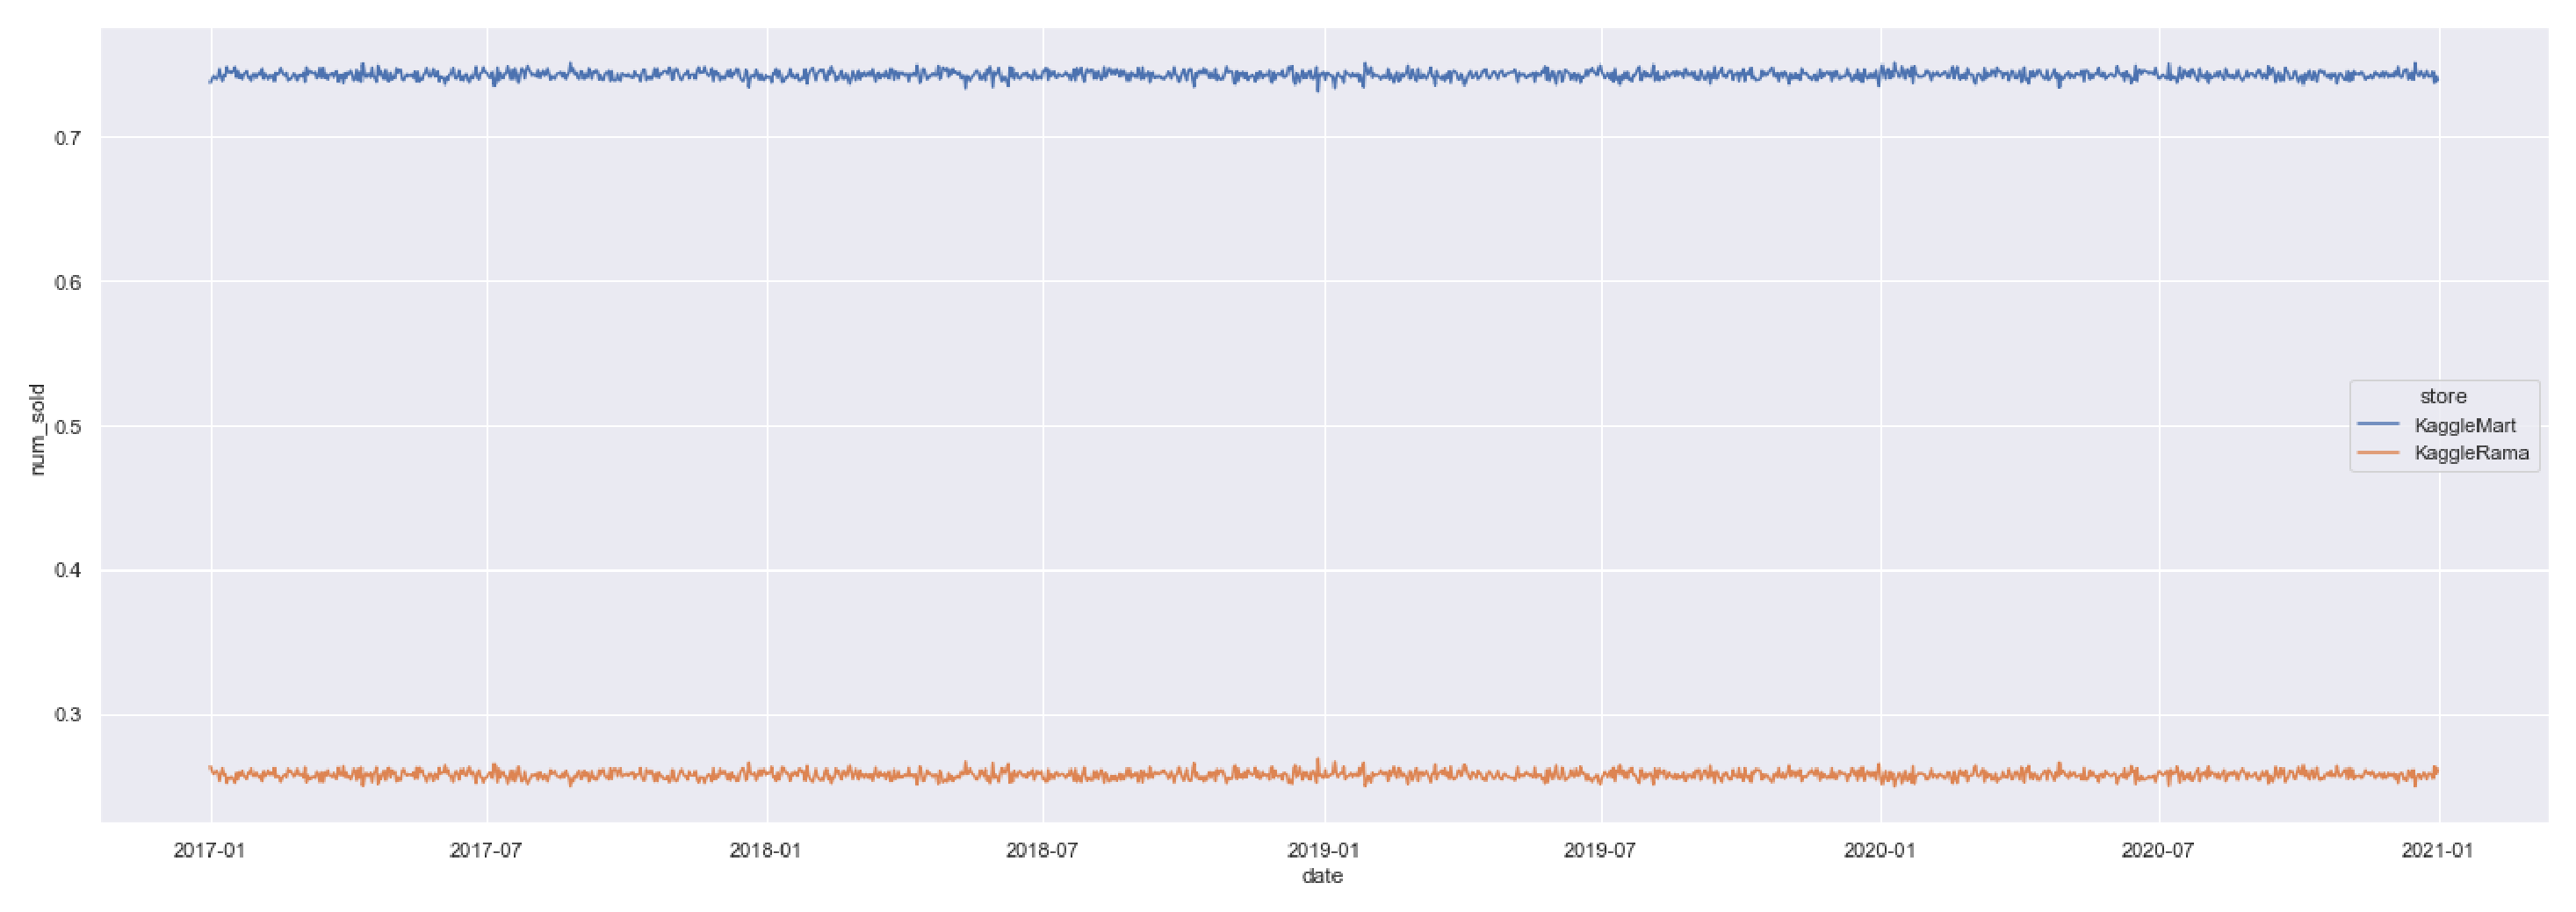
\includegraphics[width=1.1\textwidth]{store-ratio.eps}
    {\small{The trend of sales proportion in different stores}}
    \end{tikzfigure}%
    \end{minipage}
    \hfill
    \begin{minipage}{0.3\linewidth}
    \centering
    \begin{tikzfigure}
    \includegraphics[width=1.1\textwidth]{product-trend.eps}
    {\small{The trend of sales proportion for different products}}
    \end{tikzfigure}%
    \end{minipage}
\end{center}
}
%%%%%%%%%% -------------------------------------------------------------------- %%%%%%%%%%


%%%%%%%%%% -------------------------------------------------------------------- %%%%%%%%%%

%\note{Note with default behavior}

%\note[targetoffsetx=12cm, targetoffsety=-1cm, angle=20, rotate=25]
%{Note \\ offset and rotated}

 % First column - second block


%%%%%%%%%% -------------------------------------------------------------------- %%%%%%%%%%
\block{Feature Extraction}{
	Through the previous data analysis, it is found that the sales volume of stores and countries has a fixed proportion, while the sales volume of different products has a periodicity. Therefore, it is only necessary to predict
	\begin{itemize}
	\item \textcolor{red}{the total sales volume of each day.}
	\item \textcolor{red}{the sales volume of different products in each day of the year.}
	\end{itemize}
%    1) Group Feature Extraction,
%    2) Outlying Degree Scoring, and
%    3) Outlying Aspects Identification.
\begin{center}
     \begin{minipage}{0.7\linewidth}
\begin{tikzfigure}%[Overall architecture of \emph{GOAM} algorithm]
%  \includegraphics[width=0.8\linewidth]{figures//framework.pdf}
    \includegraphics[width=0.9\textwidth]{trainline.eps}
{\small{Aggregated Time Series}}
\end{tikzfigure}
		    \end{minipage}
	    \end{center}
\begin{description}
  	\item[Time Feature Extraction]
Seasonal patterns in sales were discovered through observation. We extracted features such as the month of the year, the day of the week, and the day of the year from the time series.


%    \item
%    The histogram of $G_q$ on three features are as follows.
\end{description}

\begin{center}
    \begin{minipage}{0.75\linewidth}
    \centering
    \begin{tikzfigure}
    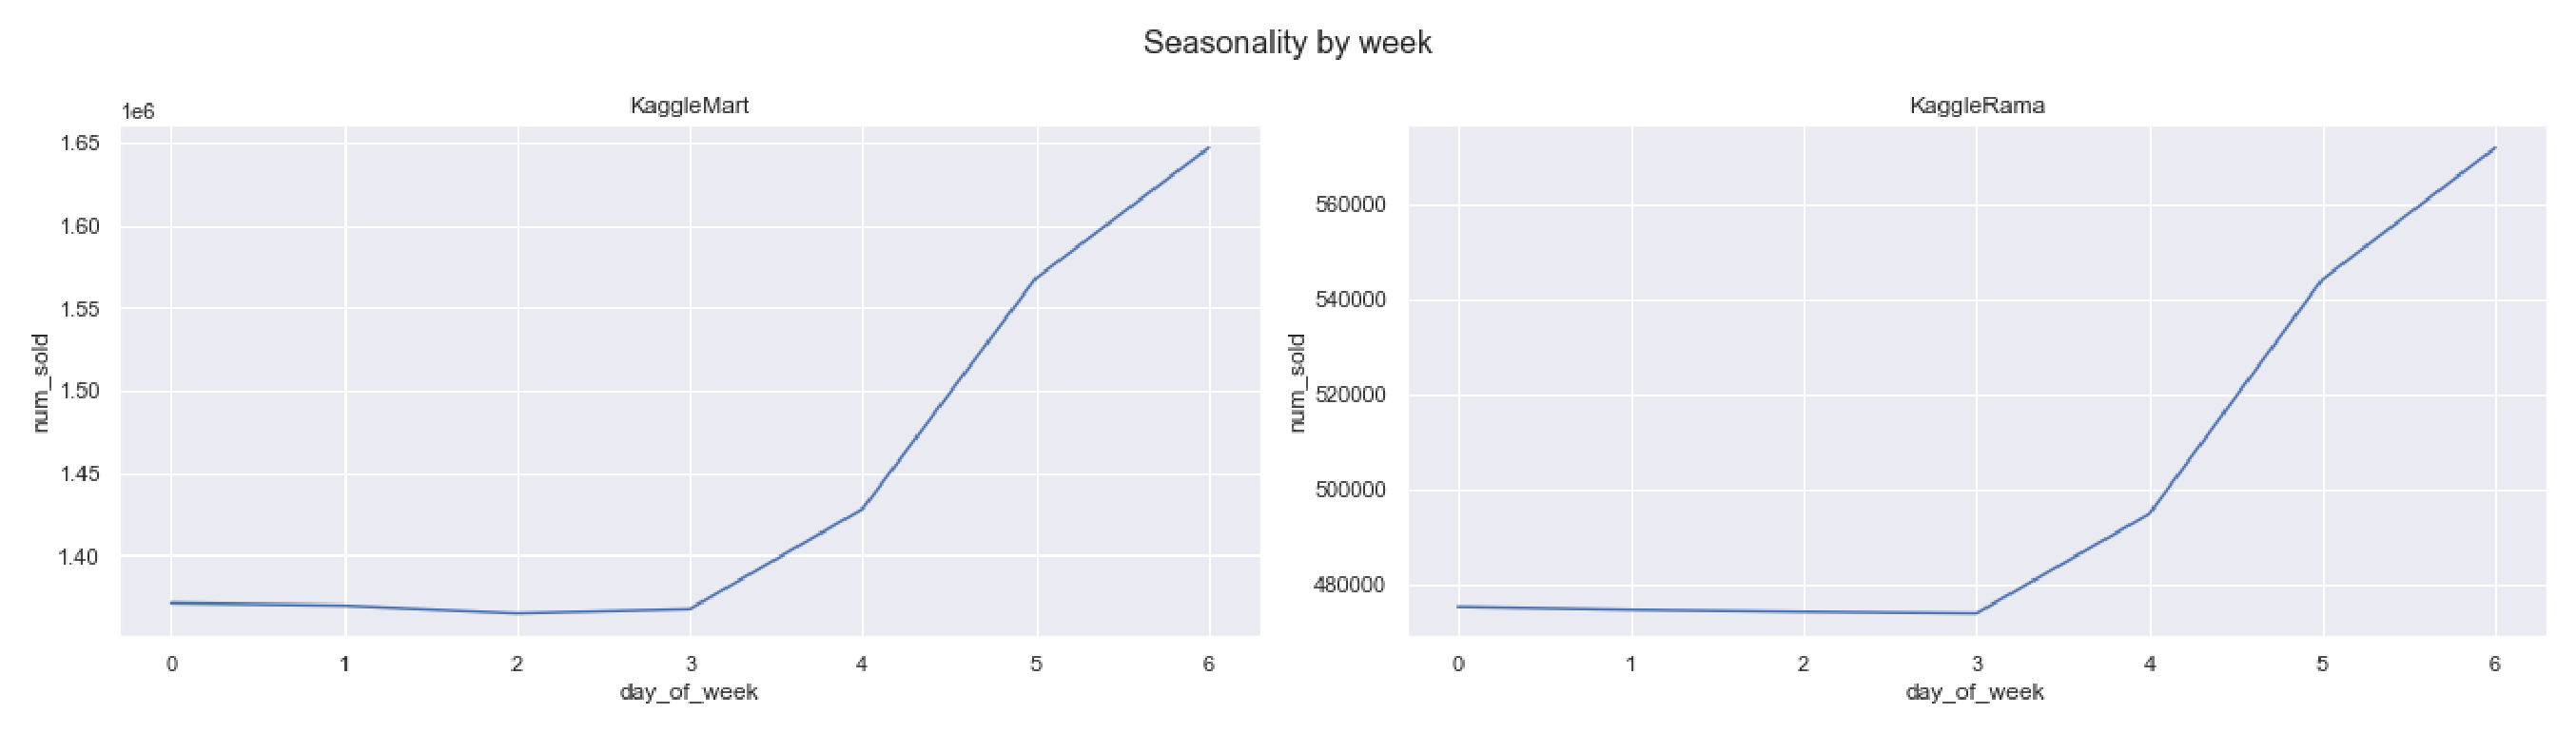
\includegraphics[width=1.05\textwidth]{week-feature.eps}
{\small{weekday feature}}
    \end{tikzfigure}%
    \end{minipage}
   
\end{center}	
\begin{description}
\item We converted the monthly data into numerical values that are suitable for input into a Fourier transform. This allows us to perform a Fourier transform on the monthly data and obtain the coefficients of the various frequency components.
\item we also took into account features related to the day of the week and important dates within the year.
\end{description}
}
%%%%%%%%%% -------------------------------------------------------------------- %%%%%%%%%%


% SECOND column
\column{0.5}
 %Second column with first block's top edge aligned with with previous column's top.

%%%%%%%%%% -------------------------------------------------------------------- %%%%%%%%%%
\block{Total Sales Forecasting}{
\begin{description}
    \item
   We use Ridge regression from the "linear\_model" module to correlate the relationship between sales and time features, and predict on the test set.
\end{description}
\begin{center}
	\begin{minipage}{0.75\linewidth}

\begin{tikzfigure}%[Overall architecture of \emph{GOAM} algorithm]
    \centering
    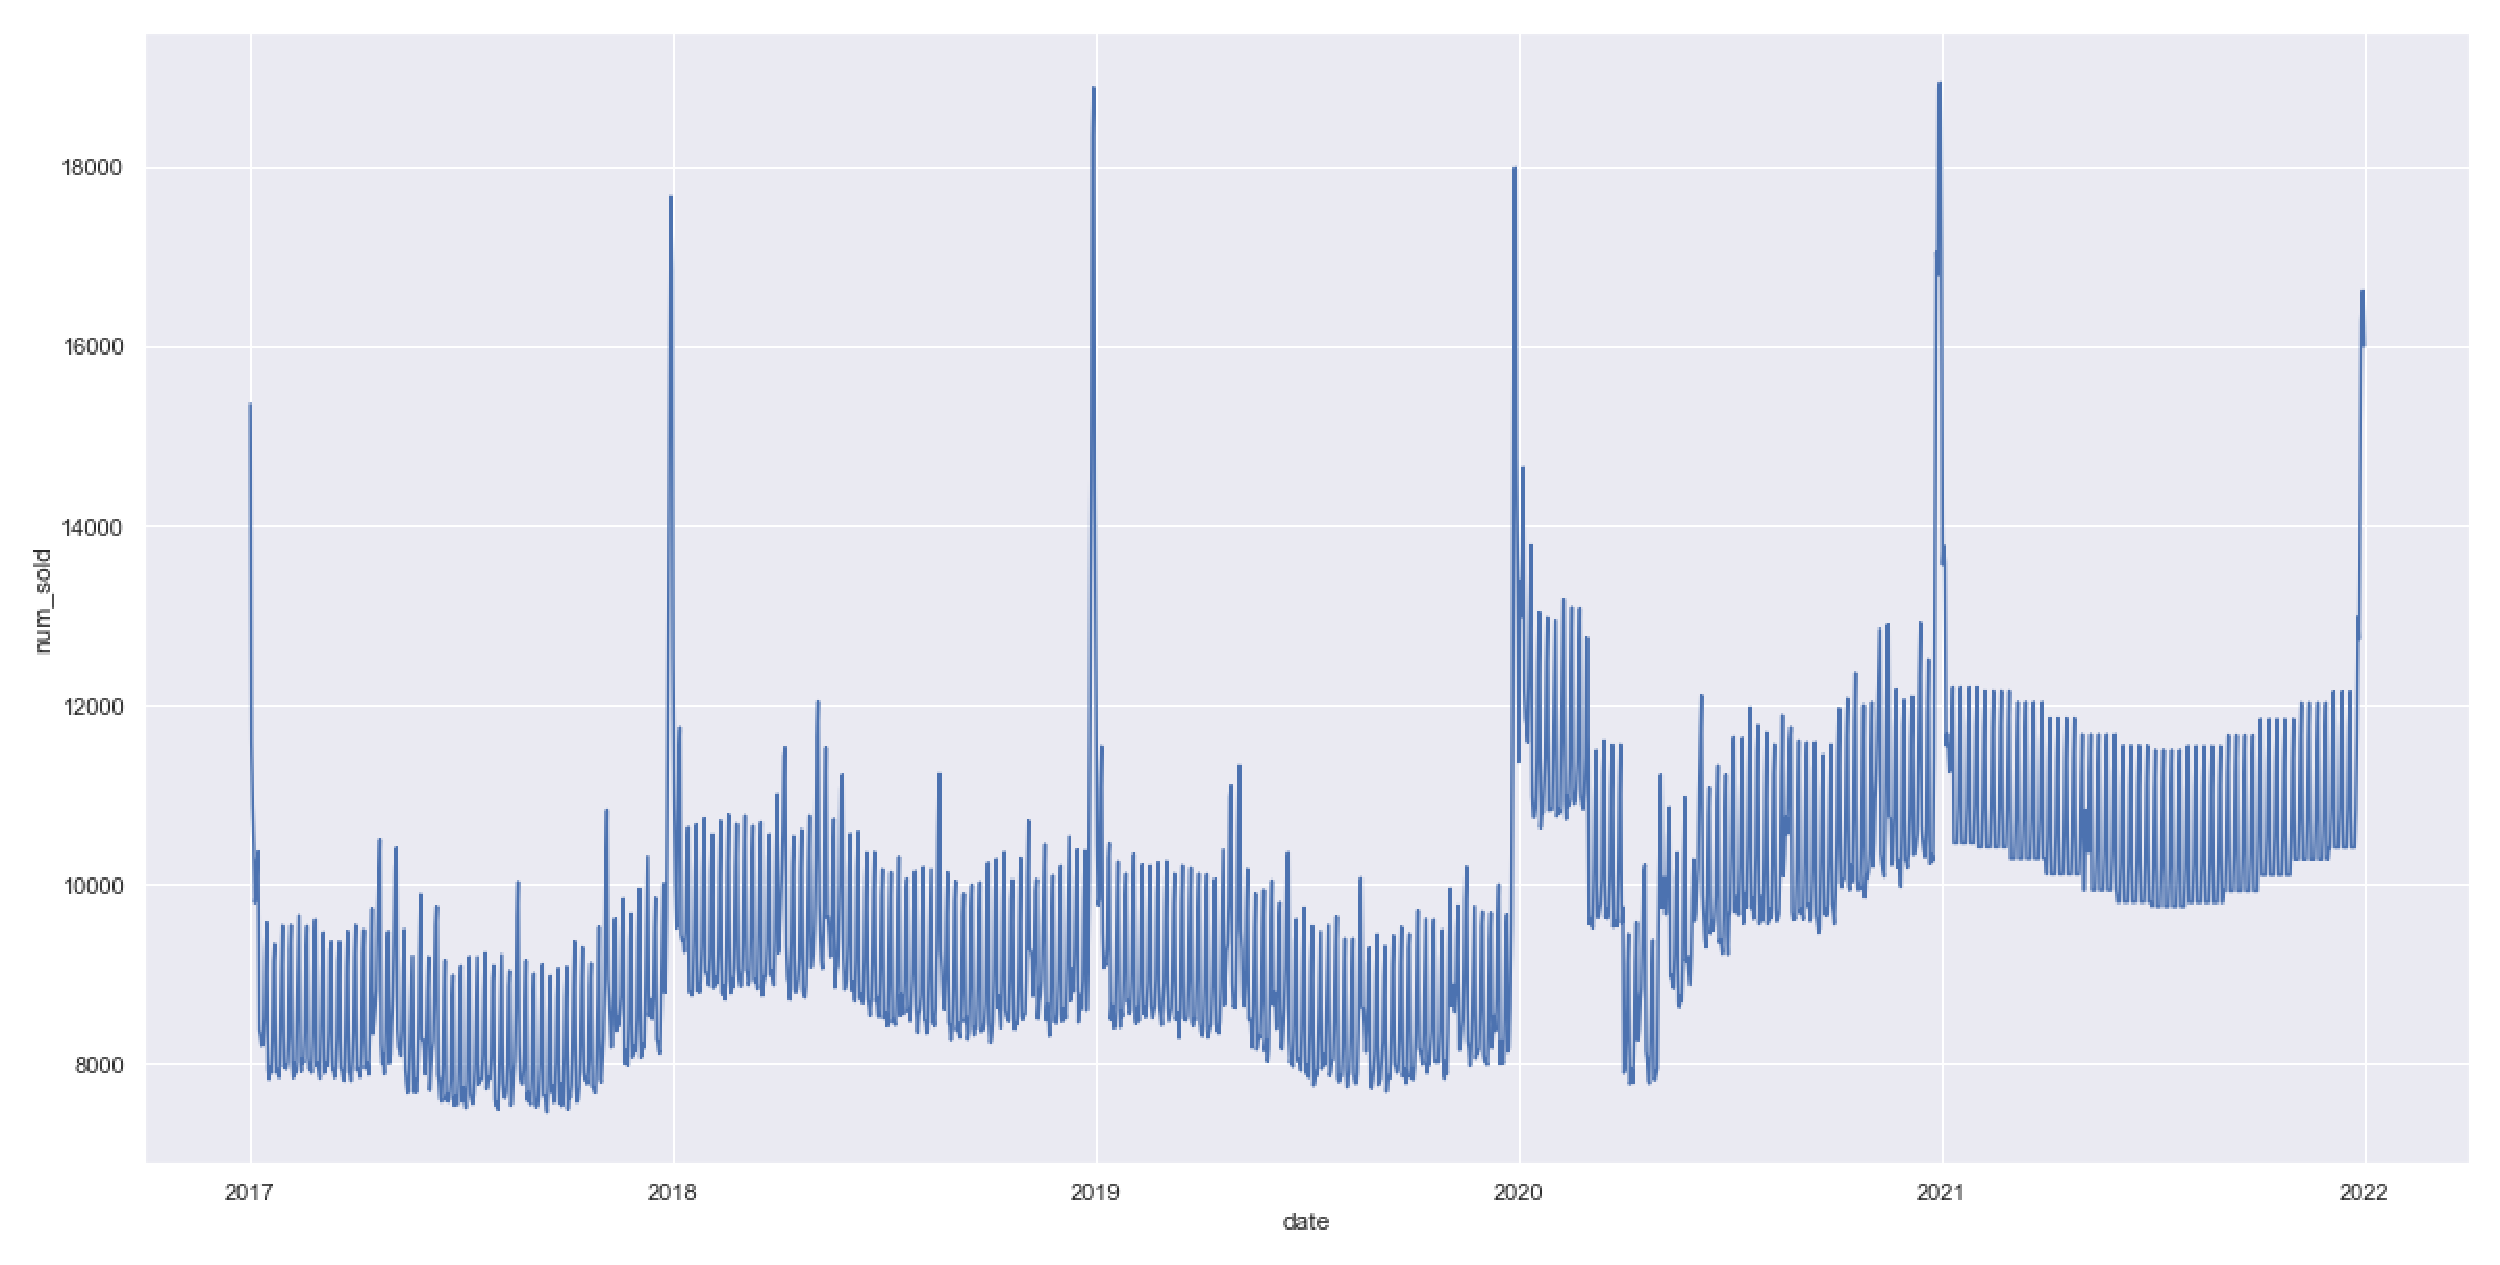
\includegraphics[width=1.05\textwidth]{total-sales.eps}
{\small{total sales forecasting}}
\end{tikzfigure}

    \end{minipage}

\end{center}	

}
%%%%%%%%%% -------------------------------------------------------------------- %%%%%%%%%%
% Second column - first block


%%%%%%%%%% -------------------------------------------------------------------- %%%%%%%%%%
\block[titleleft]{Specific Sales Forecast}
{
\begin{description}
  	\item[Product Ratio Forecast]   We found that the proportion of sales for a product has a cyclical variation with a period of two years. Therefore, we assign the daily proportion of sales for each product in 2019 to 2021.
\end{description}
\vspace{.5cm}
\begin{center}
	\begin{minipage}{0.75\linewidth}
		\centering
\begin{tikzfigure}%[Overall architecture of \emph{GOAM} algorithm]
	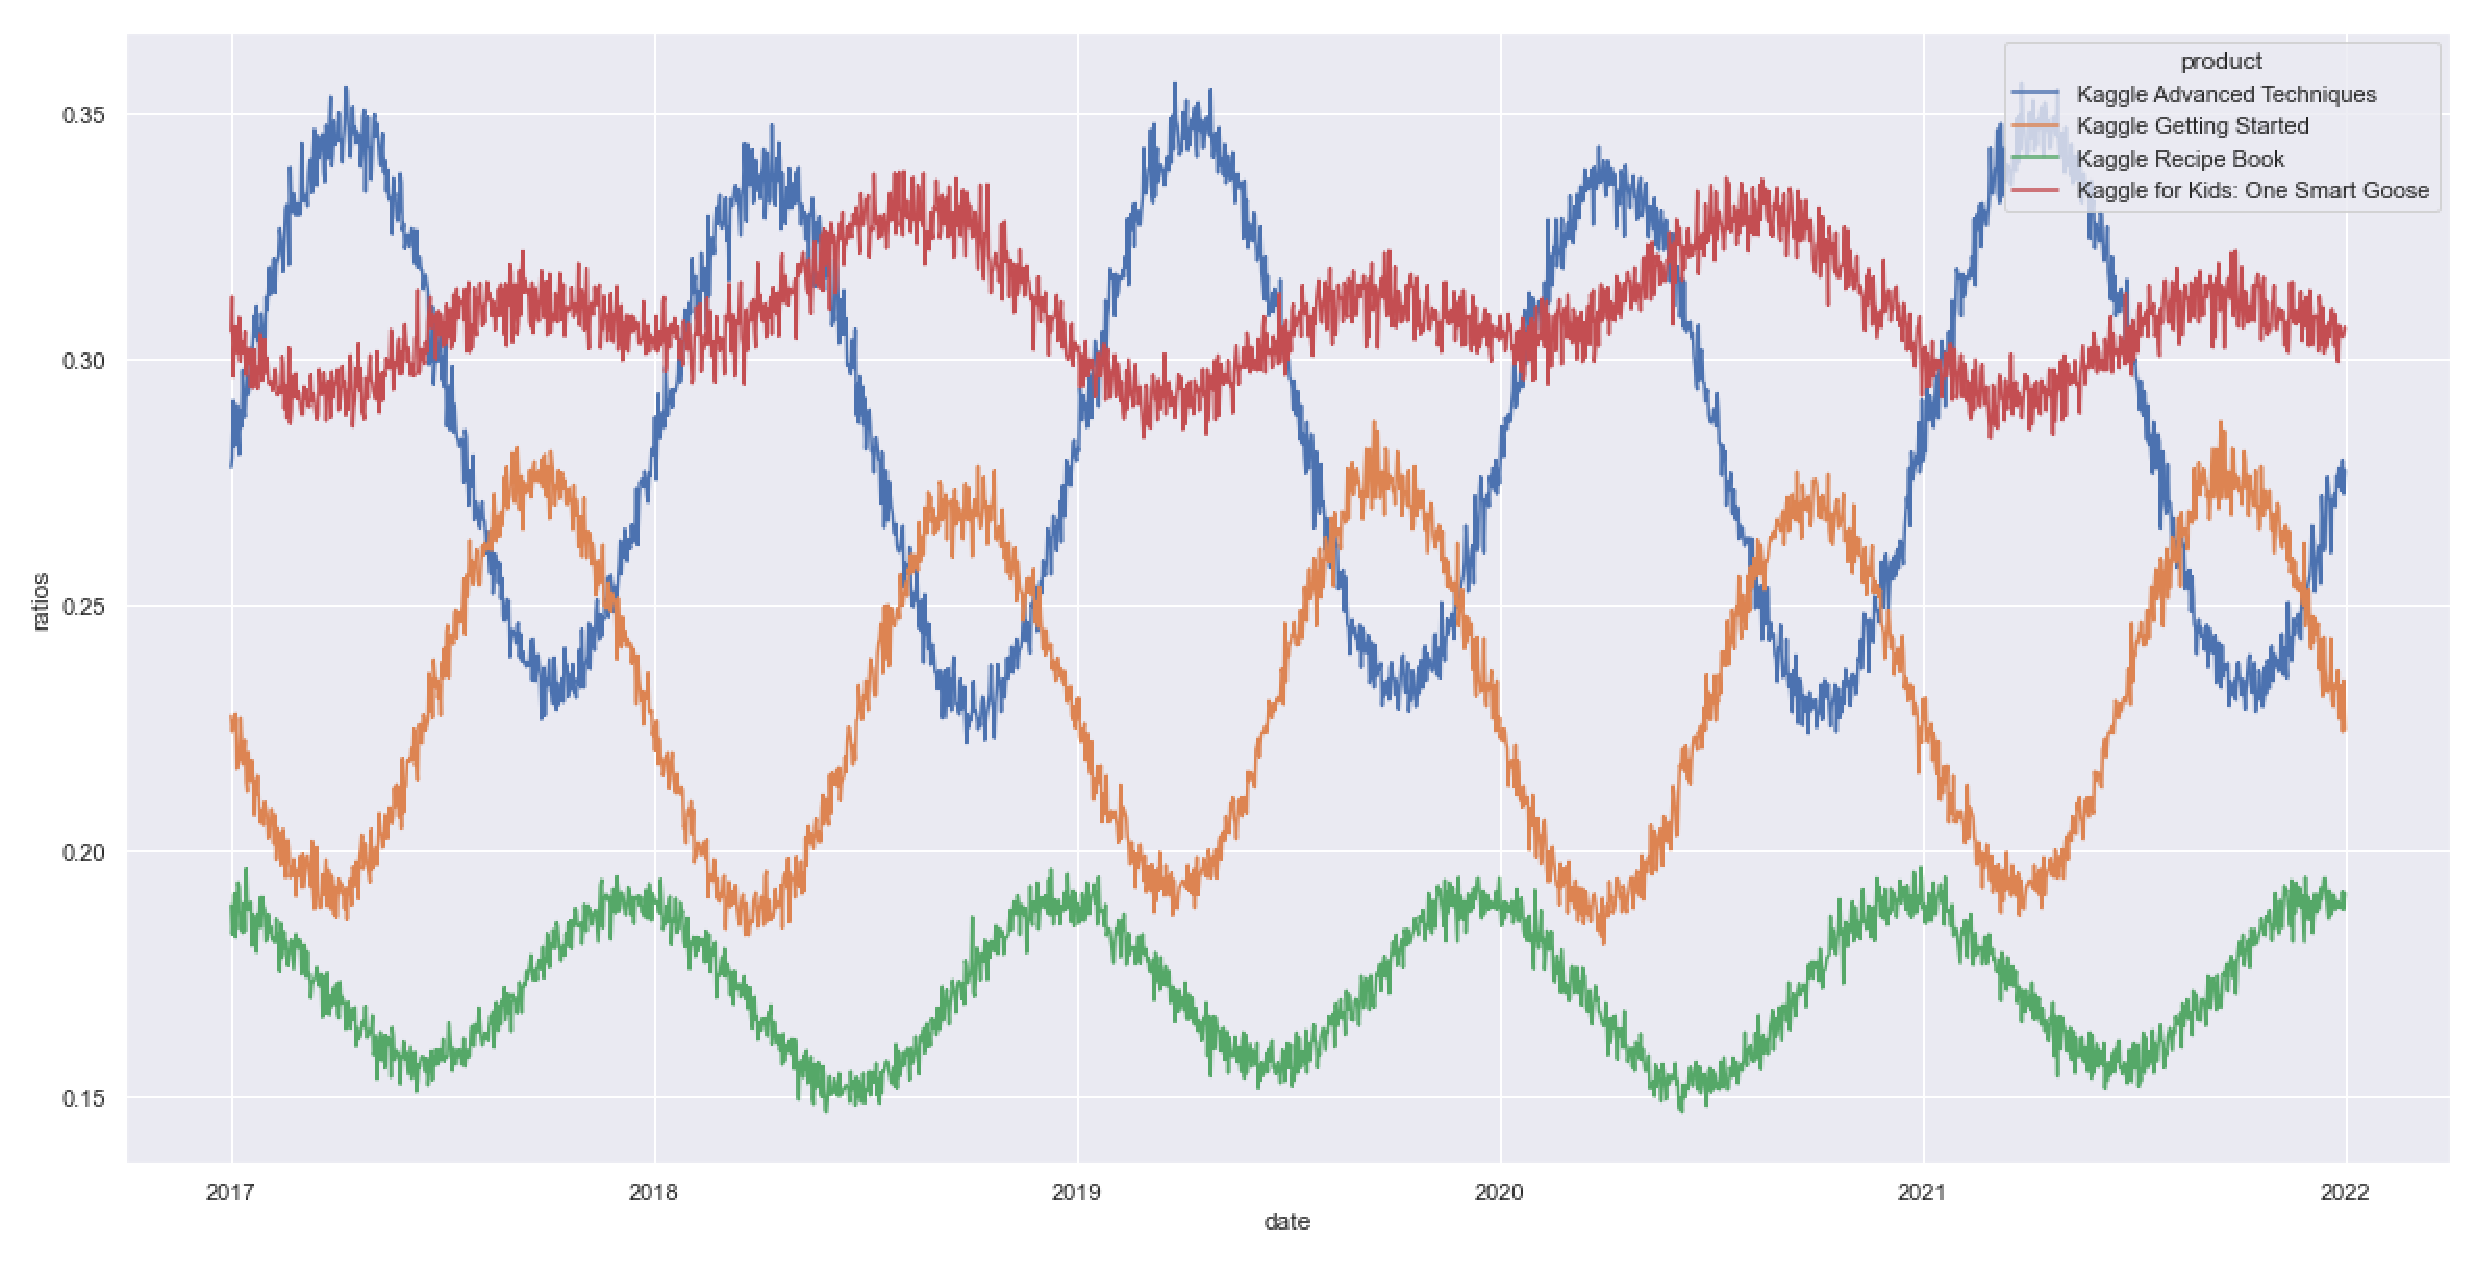
\includegraphics[width=1.1\textwidth]{product-ratio-for.eps}
	{\small{Product Ratio Forecast}}
\end{tikzfigure}
    \end{minipage}

\end{center}	

\begin{description}
\item[Country and Store Ratio Forecast]
\begin{itemize}
\item we assume that the proportion of sales in various countries in 2021 is the same as in 2020. In 2020, the proportion of sales in various countries is the same, each accounting for 1/6.
\item The proportion of different stores remains fixed, KaggleMart accounts for 75\%, and KaggleRama accounts for 25\%.
\end{itemize}
\end{description}


           \begin{center}
\begin{minipage}{0.5\linewidth}
    \centering
    \begin{tikzfigure}
	\includegraphics[width=1.1\textwidth]{final-for.eps}
{\small{Final Forecasting}}
    \end{tikzfigure}%
\end{minipage}
\end{center}
}
%%%%%%%%%% -------------------------------------------------------------------- %%%%%%%%%%


% Second column - second block
%%%%%%%%%% -------------------------------------------------------------------- %%%%%%%%%%
\block[titlewidthscale=1, bodywidthscale=1]
{Conclusion}
{
\begin{description}
  \item[Problem Definition]
  This is a time series forecasting problem that includes complex elements.

  \item[Strategies]
  Simplifying the effects of complex factors through analyzing patterns discovered through single factor analysis.
  
    \item[Prediction method]
Use linear regression method to predict the relationship between sales volume and time characteristics.
\end{description}
}
%%%%%%%%%% -------------------------------------------------------------------- %%%%%%%%%%


% Bottomblock
%%%%%%%%%% -------------------------------------------------------------------- %%%%%%%%%%


%\note[targetoffsetx=8cm, targetoffsety=-10cm,rotate=0,angle=180,radius=8cm,width=.46\textwidth,innersep=.1cm]{
%Acknowledgement
%}

%\block[titlewidthscale=0.9, bodywidthscale=0.9]
%{Acknowledgement}{
%}
%%%%%%%%%% -------------------------------------------------------------------- %%%%%%%%%%

\end{columns}


%%%%%%%%%% -------------------------------------------------------------------- %%%%%%%%%%
%[titleleft, titleoffsetx=2em, titleoffsety=1em, bodyoffsetx=2em,%
%roundedcorners=10, linewidth=0mm, titlewidthscale=0.7,%
%bodywidthscale=0.9, titlecenter]

%\colorlet{noteframecolor}{blue!20}
\colorlet{notebgcolor}{blue!20}
\colorlet{notefrcolor}{blue!20}
\note[targetoffsetx=-13cm, targetoffsety=-12cm,rotate=0,angle=180,radius=8cm,width=.96\textwidth,innersep=.4cm]
{
\begin{minipage}{0.3\linewidth}
\centering
\includegraphics[width=24cm]{./graphics/logos/tulip-wordmark.eps}
\end{minipage}
\begin{minipage}{0.7\linewidth}
{ \centering
 The $11^{th}$ International Conference on Knowledge Science,
  Engineering and Management (KSEM 2018),
  17-19/08/2018, Changchun, China
}
\end{minipage}
}
%%%%%%%%%% -------------------------------------------------------------------- %%%%%%%%%%


\end{document}

%\endinput
%%
%% End of file `tikzposter-template.tex'.
